\subsubsection{Polaganje praktičnog ispita}

\vspace{3mm}

\begin{itemize}

\item \textbf{Kratak opis:} Kandidat polaže vozački ispit i nakon uspešnog polaganja popunjava anketu o auto školi i dobija potvrdu o položenom vozačkom ispitu.

\vspace{2mm}

\item \textbf{Učesnici} \newline
   - Kandidat \newline   
   - Instruktor \newline
   - Administrativni radnik 
   
\item \textbf{Preduslovi:} \newline
   - Sistem je u funkciji. \newline
   - Kandidat se prijavio za praktični ispit.

\item \textbf{Postuslovi:} \newline
    - Kandidat je završio sa obukom.

\item \textbf{Osnovni tok:}  
   \begin{enumerate}
   \item Kandidat izlazi na završni ispit.
   \item Sistem prikazuje instruktoru putanju vožnje za tog kandidata.
   \item Instruktor saopštava putanju kandidatu.
   \item Kandidat vozi po datoj putanji.
   \item Kandidat završava ispit.
   \item Instruktor saopštava rezultate ispita.
   \begin{enumerate}
       \item Ukoliko je kandidat položio ispit, izvršava se podtok P1.
       \item Ukoliko kandidat nije položio ispit, izvršava se podtok P2.
   \end{enumerate}
   \item Sistem ažurira podatke o kandidatu.     

   \end{enumerate}

\item \textbf{Podtokovi:}   
 \begin{itemize}
   \item P1. \textbf{Kandidat je položio ispit:}
   \begin{enumerate}
       \item Instruktor unosi podatke o ispitu u sistem.
       \item Instruktor potvrđuje položen ispit u sistemu.
       \item Sistem čuva podatke o ispitu.
       \item Sistem šalje kandidatu anketu.
       \item Kandidat popunjava anketu.
       \item Sistem čuva podatke iz ankete.
       \item Administrativni radnik šalje kandidatu potvrdu o položenom vozačkom ispitu.
       \item Kandidat ulazi na mejl i proverava potvrdu o položenom vozačkom ispitu.
   \end{enumerate}
   \item P2. \textbf{Kandidat nije položio ispit:}
   \begin{enumerate}
       \item Instruktor unosi podatke o ispitu u sistem.
       \item Sistem čuva podatke o ispitu.
       \item Proces se prekida dok se kandidat opet ne prijavi za polaganje prakticnog ispita.
   \end{enumerate}
  
   \end{itemize}

\item \textbf{Alternativni tok:}  
   \begin{itemize} 
     \item A1. \textbf{Kandidat nije dobio potvrdu o položenom ispitu:}
     Administrativni radnik nije poslao potvrdu kandidatu. Kandidat obaveštava administrativnog radnika da nije dobio mejl. Proces se nastavlja u koraku 7 podtoka P1.
   \end{itemize}

\end{itemize}  

\begin{figure}[H]
  \begin{center}
      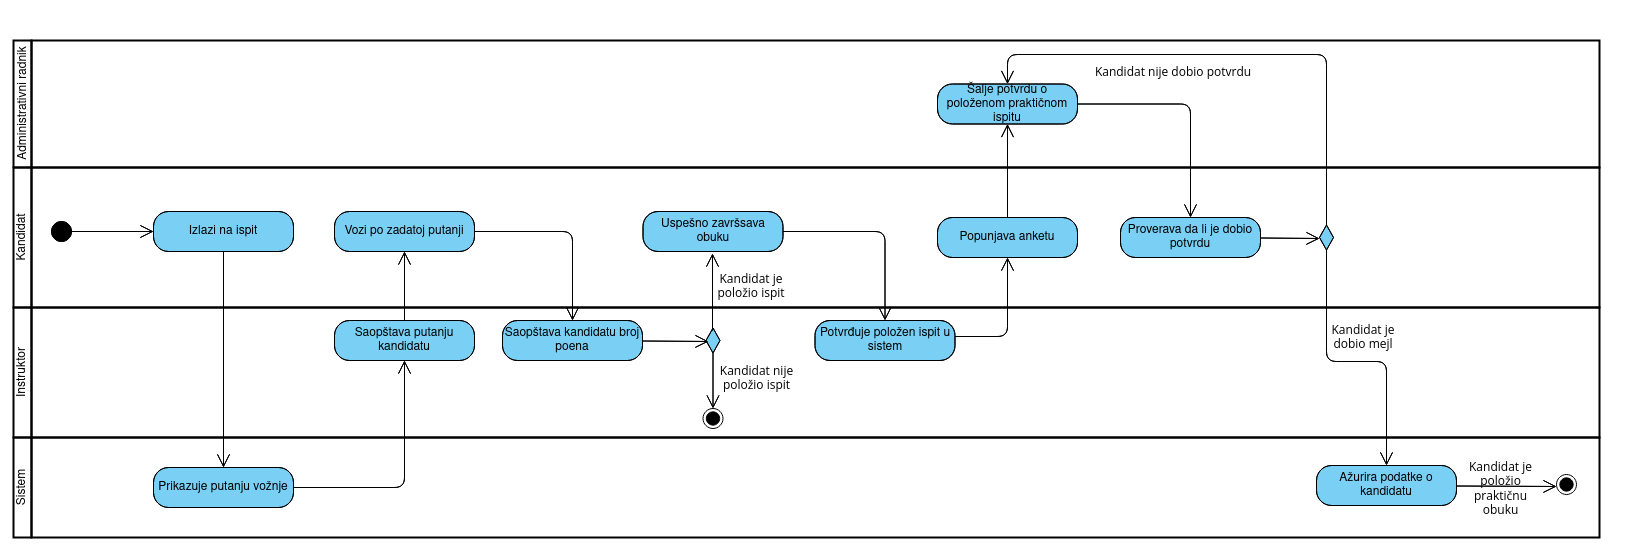
\includegraphics[width=140mm, height=70mm]{Diagrams/dijagram_aktivnosti_polaganje_prakticnog_ispita.png}
  \end{center}
  \caption {Dijagram aktivnosti - Polaganje praktičnog ispita}
  \label{activity_polaganje_praktičnog_ispita}

\end{figure}
